\documentclass[11pt]{article}

\usepackage{amsmath}
\usepackage{bm} % For \boldmath command
\usepackage{booktabs}
\usepackage{enumitem}
\usepackage[margin=1in]{geometry}
\usepackage{libertine}
\usepackage[libertine]{newtxmath}
\usepackage{pgfplots}
\usepackage{siunitx}

\pgfplotsset{compat=1.16}
\usetikzlibrary{arrows.meta}
\usetikzlibrary{bending} % For 'flex' option on arrow tips
\usetikzlibrary{calc}
\usetikzlibrary{decorations}
\usetikzlibrary{positioning}
\pgfarrowsdeclarecombine{dist}{dist}{stealth}{stealth}{|}{|}

\sisetup{separate-uncertainty=true}

\title{Experiment 6: Simple Harmonic Motion}
\author{
    Brandon Tsang \\
    PHYS 122L-002
}
\date{January 15, 2020}

\begin{document}
\maketitle
\section*{Part 1: Simple Harmonic Motion on a Linear Air Track}
    \subsection*{Experiment Summary}
        In this experiment, we will demonstrate the equations of simple harmonic motion using a setup as illustrated below:
        \vspace{\abovedisplayskip}
        \begin{center}
            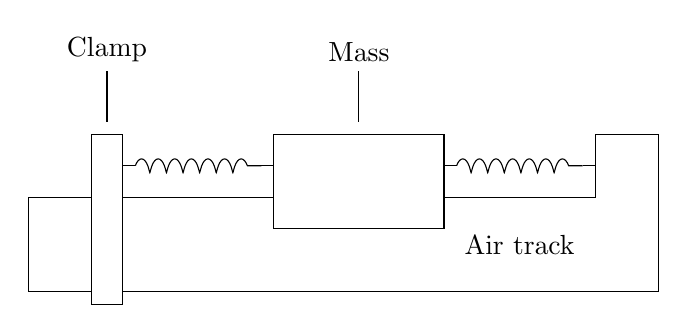
\begin{tikzpicture}[scale=0.8]
                % Air track
                \draw (0,0)
                    -- ++(10,0)
                    -- ++(0,2.5)
                    -- ++(-1,0)
                    -- ++(0,-1)
                    -- (0,1.5)
                    -- cycle;
                
                \draw[fill=white] (1,-0.2) rectangle (1.5,2.5); % Clamp
                
                % Left spring
                \draw (1.5,2) -- ++(0.2,0);
                \draw[decorate, decoration={coil, segment length=6, aspect=0.3}] (1.7,2) -- ++(2,0);
                \draw (3.7,2) -- ++(0.2,0);
                
                \draw[fill=white] (3.9,1) rectangle (6.6,2.5); % Mass
                
                % Right spring
                \draw (6.6,2) -- ++(0.2,0);
                \draw[decorate, decoration={coil, segment length=6, aspect=0.3}] (6.8,2) -- ++(2,0);
                \draw (8.8,2) -- ++(0.2,0);
                
                % Labels
                \node at (7.8,0.75) {Air track};
                \draw (1.25,2.7) -- ++(0,0.8)
                    node[anchor=south] {Clamp};
                \draw (5.25,2.7) -- ++(0,0.8)
                    node[anchor=south] {Mass};
            \end{tikzpicture}
        \end{center}
        \vspace{\belowdisplayskip}
        The mass is suspended by two strings over an air track, which minimizes friction. The two springs are somewhat stretched. The mass is then moved and it oscillates as it tries to return to its equilibrium position. This oscillation's period is measured, and, along with the mass of the mass, is used to calculate the spring constant $k$ with the equation
        \begin{equation}
            \label{eqn:spring}
            T=2\pi\sqrt{\frac{m}{k}}
        \end{equation}
        \par
        To confirm the value of $k$ obtained from the experiment, we will perform a second, smaller experiment where we suspend masses from one of the springs from the original experiment, and determine $k$ again.
    \subsection*{Results}
        Graphs for our data are at the end of the document.
        \begin{center}
            \begin{tabular}{c l l l l l}
                \toprule
                Cart \# & \multicolumn{1}{c}{Mass ($m$)} & \multicolumn{1}{c}{$\omega$} & \multicolumn{1}{c}{Period ($T$)} & \multicolumn{1}{c}{$T^2$} & \multicolumn{1}{c}{Graph} \\
                \midrule
                1 & \SI{0.518(3)}{\kilogram} & \SI{4.5(3)}{\per\second} & \SI{1.393(1)}{\second} & \SI{1.9409(3)}{\square\second} & Figure~\ref{fig:blue-glider} \\
                2 & \SI{0.657(7)}{\kilogram} & \SI{4.0(4)}{\per\second} & \SI{1.567(2)}{\second} & \SI{2.455(6)}{\square\second} & Figure~\ref{fig:blue-white-glider} \\
                3 & \SI{0.822(5)}{\kilogram} & \SI{3.6(4)}{\per\second} & \SI{1.750(2)}{\second} & \SI{3.063(6)}{\square\second} & Figure~\ref{fig:blue-red-glider} \\
                \bottomrule
            \end{tabular}
        \end{center}
        \vspace{\belowdisplayskip}
        We can rearrange Equation~\ref{eqn:spring} as follows:
        \begin{align}
            T&=2\pi\sqrt{\frac{m}{k}} \\
            T^2&=\frac{4\pi^2}{k}m \label{eqn:rearranged-spring}
        \end{align}
        Equation~\ref{eqn:rearranged-spring} is of the form $y=mx+b$, so we can plot a graph of $T^2$ vs. $m$. The slope of the line produced will be equal to $\frac{4\pi^2}{k}$. (The error bars in the graph below are too small to be visible)
        \vspace{\abovedisplayskip}
        \begin{center}
            \begin{tikzpicture}
                \begin{axis}[
                    axis lines=left,
                    axis line style={shorten >=-10pt},
                    xmin=0, xmax=1.5,
                    ymin=0,
                    xlabel=$m$,
                    ylabel=$T^2$,
                    grid=both,
                    legend entries={$3.69092x+0.0293744$}
                ]
                    \addplot[
                        black, mark=*,
                        forget plot,
                        error bars/.cd,
                        x dir=both, x explicit,
                        y dir=both, y explicit
                    ]
                        table[
                            x=m, y=t2, col sep=comma,
                            x error=m-error,
                            y error=t2-error
                        ]
                        {res/data1.csv};
                    \addplot[black!50, mark=none, dashed]
                        {3.69092*x+0.0293744};
                \end{axis}
            \end{tikzpicture}
        \end{center}
        The slope of the line is 3.69092, so we can now calculate $k$. Since the experiment had two springs, this value will actually be twice the real value of $k$. We will replace $k$ with $2k$ and proceed:
        \begin{align}
            3.69092&=\frac{4\pi^2}{2k} \\
            2k&=\frac{4\pi^2}{3.69092} \\
            2k&=10.696 \\
            k&=5.348
        \end{align}
        To confirm the value of $k$, we suspend different masses on one of the springs from the previous portion of the experiment, and measure the spring extension. Using $mg=kx$, we can can calculate the spring constant once more.
        \begin{center}
            \begin{tabular}{l l l}
                \toprule
                \multicolumn{1}{c}{Mass} & \multicolumn{1}{c}{Spring extension} & \multicolumn{1}{c}{$k$} \\
                \midrule
                \SI{10}{\gram} & \SI{1.7(1)}{\centi\meter} & \SI{5.70(6)}{} \\
                \SI{20}{\gram} & \SI{3.4(1)}{\centi\meter} & \SI{5.70(6)}{} \\
                \SI{30}{\gram} & \SI{5.3(1)}{\centi\meter} & \SI{5.50(4)}{} \\
                \SI{40}{\gram} & \SI{7.3(1)}{\centi\meter} & \SI{5.30(7)}{} \\
                \bottomrule
            \end{tabular}
        \end{center}
        The average $k$ value is \SI{5.6(1)}{}.
    \subsection*{Discussion}
        \begin{enumerate}
            \item{
                \textbf{How do your results for the spring constant compare? Do you results agree within experimental uncertainty?}
                \par
                The percent difference between the two $k$ values is 3.7\%. We had no time to calculate the uncertainty, so we don't know if the results fall within with predicted uncertainties.
            }
            \item{
                \begin{enumerate}
                    \item{
                        \textbf{Does the theory explain the experimental results? (i.e. is the relationship between the period and the mass correctly described by the equations?)}
                        \vspace{\abovedisplayskip}
                        \begin{center}
                            \begin{tabular}{c l l l}
                                \toprule
                                Cart \# & \multicolumn{1}{c}{Mass ($m$)} & \multicolumn{1}{c}{Period ($T$)} & \multicolumn{1}{c}{$2\pi\sqrt{\frac{m}{k}}$} \\
                                \midrule
                                1 & \SI{0.518(3)}{\kilogram} & \SI{1.393(1)}{\second} & \SI{1.955}{\second} \\
                                2 & \SI{0.657(7)}{\kilogram} & \SI{1.567(2)}{\second} & \SI{2.202}{\second}\\
                                3 & \SI{0.822(5)}{\kilogram} & \SI{1.750(2)}{\second} & \SI{2.463}{\second} \\
                                \bottomrule
                            \end{tabular}
                        \end{center}
                        \vspace{\belowdisplayskip}
                        The predicted periods tend to be consistently higher than the measured periods. This could be due to an error in calculating the $k$ values messing up the predicted periods.
                    }
                    \item{
                        \textbf{Is your graph well described by a stright line, or is there evidence for errors? Can you identify the errors?}
                        The graph is almost exactly a straight line (albeit with only three data points), and the error bars are so small they are not visible.
                    }
                    \item{
                        \textbf{What is the intercept? Is it zero? Should it be?}
                        The intercept is \~0.029, which is very close to zero. It should be zero since $T^2=\frac{4\pi^2}{k}m$, and when $m$ is zero, $T^2$ is also zero.
                    }
                \end{enumerate}
            }
            \item{
                \textbf{Compare the methods used for extracting the period of the periodic motion using Pasco Capstone to the method of extracting the period from the time duration for a known number of oscillations. Are there significant differences? Should one method be preferred over another? If so, why?}
            }
        \end{enumerate}
\section*{Part 2: Rotational Simple Harmonic Motion}
    \subsection*{Experiment Summary}
        In this experiment, a torsion pendulum will be set up as illustrated below:
        \vspace{\abovedisplayskip}
        \begin{center}
            \begin{tikzpicture}[
                x={(0.866cm,0.5cm)}, y={(-0.866cm,0.5cm)}, z={(0cm,1cm)},
                scale=0.8
            ]
                % Box
                \draw[black!50] (0,0,4)
                    -- ++(1,0,0)
                    -- ++(0,0,0.3)
                    -- ++(0,1,0)
                    -- ++(-1,0,0)
                    -- ++(0,0,-0.3)
                    -- ++(0,-1,0)
                    -- ++(0,0,0.3)
                    -- +(0,1,0)
                    +(0,0,0)
                    -- +(1,0,0);
                \draw (0,0,4) -- (0,0,0); % String
                
                % Labels behind
                \draw[{dist[slant=0.6]}-{dist[slant=0.6]}] (-0.5,3.5,-0.5) -- (-0.5,0,-0.5)
                    node[midway, anchor=north east] {$r$};
                \draw[{dist[slant=0.6]}-{dist[slant=0.6]}] (-1.5,-5,-0.5) -- (-1.5,5,-0.5)
                    node[midway, anchor=north east] {$l$};
                
                % Rotated rod
                \begin{scope}[black!30]
                    % Far rod segment
                    \draw (2.5,4.33,0) circle[radius=2.5pt];
                    \draw[double=white, double distance=4pt] (2.5,4.33,0) -- (2,3.464,0);
                    
                    \draw[fill=white] (1.75,3,0) circle[radius=0.5cm]; % Far ball
                    
                    % Middle rod segment
                    \draw (1.6,2.77,0) circle[radius=2.5pt];
                    \draw[double=white, double distance=4pt] (1.6,2.77,0) -- (-1.75,-3,0);
                    
                    \draw[fill=white] (-1.75,-3,0) circle[radius=0.5cm]; % Near ball
                    
                    % Near rod segment
                    \draw (-1.9,-3.29,0) circle[radius=2.5pt];
                    \draw[double=white, double distance=4pt] (-1.9,-3.29,0) -- (-2.5,-4.33,0);
                    \draw (-2.5,-4.33,0) circle[radius=2.5pt];
                \end{scope}
                
                % Far rod segment
                \draw (0,5,0) circle[radius=2.5pt];
                \draw[double=white, double distance=4pt] (0,5,0) -- (0,4,0);
                
                \draw[fill=white] (0,3.5,0) circle[radius=0.5cm]
                    node[above=0.5cm] {$m$}; % Far ball
                
                % Middle rod segment
                \draw (0,3.2,0) circle[radius=2.5pt];
                \draw[double=white, double distance=4pt] (0,3.2,0) -- (0,-3.5,0);
                
                \draw[fill=white] (0,-3.5,0) circle[radius=0.5cm]
                    node[above=0.5cm] {$m$}; % Near ball
                
                % Near rod segment
                \draw (0,-3.8,0) circle[radius=2.5pt];
                \draw[double=white, double distance=4pt] (0,-3.8,0) -- (0,-5,0)
                    node[anchor=west] {$M$};
                \draw (0,-5,0) circle[radius=2.5pt];
                
                % Labels in front
                \draw[-{Stealth[flex]}] (0.3,0,1) arc (0:300:0.3)
                    node[anchor=west] {$K$};
                \draw[-Stealth] (0,2,0) arc (90:60:2)
                    node[midway, anchor=south] {$\theta$};
            \end{tikzpicture}
        \end{center}
        \vspace{\belowdisplayskip}
        Once the rod is rotated by some angle $\theta$, it will start rotating back and forth, causing a torsion $K$ on the string. We will measure the period of oscillation, and use the equation
        \begin{equation}
            T=2\pi\sqrt{\frac{I_c}{K}}
        \end{equation}
        to solve for this torsion.
    \subsection*{Results}
        {
            \raggedright
            The mass of the rod, $M$, is \SI{1.326(2)}{\kilo\gram}. \\
            The mass of the weights, $m$, is \SI{500}{\gram}. \\
            The length of the rod, $l$, is \SI{0.994(1)}{\meter}.
        \begin{center}
            \begin{tabular}{c l l l}
                \toprule
                Trial \# & \multicolumn{1}{c}{Distance of mass ($r$)} & \multicolumn{1}{c}{Moment of inertia ($I$)} & \multicolumn{1}{c}{Period ($T$)}\\
                \midrule
                1 & \SI{10}{\centi\meter} & \SI{0.119}{\kilogram\meter\squared} & \SI{0.58(1)}{\second} \\
                2 & \SI{20}{\centi\meter} & \SI{0.149}{\kilogram\meter\squared} & \SI{0.67(1)}{\second} \\
                3 & \SI{30}{\centi\meter} & \SI{0.199}{\kilogram\meter\squared} & \SI{0.77(1)}{\second} \\
                4 & \SI{40}{\centi\meter} & \SI{0.269}{\kilogram\meter\squared} & \SI{0.88(1)}{\second}\\
                \bottomrule
            \end{tabular}
        \end{center}
        We are given two equations:
        \begin{equation}
            T=2\pi\sqrt{\frac{I_c}{K}}
        \end{equation}
        and
        \begin{equation}
            I_c=\frac{1}{12}Ml^2+2mr^2
        \end{equation}
        Combining these, we get
        \begin{align}
            T&=2\pi\sqrt{\frac{\frac{1}{12}Ml^2+2mr^2}{K}} \\
            T^2&=4\pi\left(\frac{\frac{1}{12}Ml^2+2mr^2}{K}\right) \\
            &=\frac{\pi Ml^2}{3K}+\frac{8\pi m}{K}r^2
        \end{align}
        If we realize that the variables here are $T^2$ and $r^2$, we can see that this equation is too of the form $y=mx+b$ and can be graphed as a line where $\frac{8\pi m}{K}$ is the slope and $\frac{\pi Ml^2}{3K}$ is the $y$-intercept:
        \vspace{\abovedisplayskip}
        \begin{center}
            \begin{tikzpicture}
                \begin{axis}[
                    ymin=0, ymax=4.5,
                    axis lines=left,
                    axis line style={shorten >=-10pt},
                    xlabel=$r^2$,
                    ylabel=$T^2$
                ]
                    \addplot[
                        black, mark=*,
                        error bars/.cd,
                        x dir=both, x explicit,
                        y dir=both, y explicit
                    ]
                        table[
                            x=mr2, y=t2, col sep=comma,
                            x error=mr2-error, y error=t2-error
                        ]
                        {res/data2.csv};
                    \addplot[black!50, mark=none, dashed]
                        coordinates {(0,1) (5,3.5)};
                \end{axis}
            \end{tikzpicture}
        \end{center}
    \subsection*{Discussion}
        \begin{enumerate}
            \item{
                \textbf{How well does the theory describe the relationship between period and moment of inertia for this rotational system?}
            }
            \item{
                \textbf{What level of agreement is there between the value for the moment of inertia obtained from the graph and that computed directly?}
            }
        \end{enumerate}
\newpage
\section*{Raw Data}
\begin{figure}[h]
    \centering
    \caption{Position vs. time for blue glider only}
    \label{fig:blue-glider}
    \begin{tikzpicture}
        \begin{axis}[
            xmin=0, xmax=10,
            enlarge y limits=1,
            width=0.8\textwidth, height=2in,
            xlabel={Time (\si{\second})},
            ylabel={Position (\si{\meter})},
            legend entries={$-0.0518\sin(4.51x+7.98)+2.06$}
        ]
            \addplot[mark=none, forget plot]
                table[
                    x=Time, y=Position,
                    col sep=comma
                ]
                {res/blue-glider.csv};
            \addplot[red, dashed, mark=none, domain=0:10, samples=100]
                {-0.0518*sin(deg(4.51*x+7.98))+2.06};
        \end{axis}
    \end{tikzpicture}
\end{figure}
\begin{figure}[h]
    \centering
    \caption{Position vs. time for blue and white glider}
    \label{fig:blue-white-glider}
    \begin{tikzpicture}
        \begin{axis}[
            xmin=0, xmax=10,
            enlarge y limits=1,
            width=0.8\textwidth, height=2in,
            xlabel={Time (\si{\second})},
            ylabel={Position (\si{\meter})},
            legend entries={$0.0499\sin(4.01x+4.83)+2.06$}
        ]
            \addplot[mark=none, forget plot]
                table[
                    x=Time, y=Position,
                    col sep=comma
                ]
                {res/blue-white-glider.csv};
            \addplot[red, dashed, mark=none, domain=0:10, samples=100]
                {0.0499*sin(deg(4.01*x+4.83))+2.06};
        \end{axis}
    \end{tikzpicture}
\end{figure}
\begin{figure}[h]
    \centering
    \caption{Position vs. time for blue and red glider}
    \label{fig:blue-red-glider}
    \begin{tikzpicture}
        \begin{axis}[
            xmin=0, xmax=10,
            enlarge y limits=1,
            width=0.8\textwidth, height=2in,
            xlabel={Time (\si{\second})},
            ylabel={Position (\si{\meter})},
            legend entries={$0.0507\sin(3.59x+4.91)+2.06$}
        ]
            \addplot[mark=none, forget plot]
                table[
                    x=Time, y=Position,
                    col sep=comma
                ]
                {res/blue-red-glider.csv};
            \addplot[red, dashed, mark=none, domain=0:10, samples=100]
                {0.0507*sin(deg(3.59*x+4.91))+2.06};
        \end{axis}
    \end{tikzpicture}
\end{figure}
\end{document}
